\chapter{The refinement algorithm}

The given theory then lead to the development of a program
implementing an algorithm for solving the refinement problem on mvPDA.
This program should eventually be integrated into the MoTraS tool
for modal transitions systems \cite{Stoll11}.
Therefore, to maintain cross-platform compatibility, it
is written in Scala and Java, which allows to run on the JVM.
The program can also be used as a standalone tool
from the command line.

The basic idea of the algorithm is computing the set of all
attack rules for a given mvPDA, by which it can decide refinement.
Here the parts of the program are described as well as
some finer implementation details, the basic usage and
the performance results of several benchmarks is shown.

\section{Implementation}

The main entry point is the function {\scfont{mvPDARefinement}} shown
in pseudocode in figure \ref{alg:mvpad-refining}.
It takes as input two processes $P⋅S$, $Q⋅T$ and an mvPDA.
Then it initialises the rules with the set of basic rules and enters a loop.
As long as there are two rules in the set of rules such that they can be combined
into new rules, which are not completely contained in the set of rules, the new rules
will be added.
This will compute the fixed point of the rules under the combination of rules.
Then it returns if the refinement $P⋅S ≤_m Q⋅T$ holds by testing if the empty
rule from the initial state is contained in the rules.

\begin{figure}[H]
\begin{algorithmic}[1]
\Function{mvPDARefinement}{$P⋅S, Q⋅T, mvPDA$}
  \State $initial ← (P⋅S, Q⋅T)$
  \State $rules ← \Call{makeRules}{mvPDA}$
  \While{$\exists lhsRule, rhsRule ∈ rules :
      \Call{Combine}{lhsRule, rhsRule} ⊄ rules $}
    \State $rules ← rules ∪ \Call{combine}{lhsRule, rhsRule}$
  \EndWhile
  \State \textbf{return} $(initial, ∅) ∈ rules$
\EndFunction
\end{algorithmic}
\caption{Algorithm for testing refinement on an mvPDA}
\label{alg:mvpad-refining}
\end{figure}

\begin{figure}[H]
\begin{algorithmic}[1]
\Function{makeRules}{$mvPDA = (\Dmay, \Dmust)$}
  \State $rules ← ∅$
  \For{$P,Q,S,T ∈ Const(mvPDA), a ∈ Act(mvPDA)\}$}
    \LineComment{Attack from left-hand side for may rules}
      \State $lhs ← (P⋅S, Q⋅T)$
      \For{$(P⋅S, a, p') ∈ \Dmay$}
        \State $rhs ← ∅$
        \For{$(Q⋅T, a, q') ∈ \Dmay$}
          \State $rhs ← rhs ∪ \{ (p', q') \}$
        \EndFor
        \State $rules ← rules ∪ \{(lhs, rhs)\}$
      \EndFor
    \LineComment{Attack from right-hand side for must rules}
      \State $lhs ← (Q⋅T, P⋅S)$
      \For{$(Q⋅T, a, q') ∈ \Dmust$}
        \State $rhs ← ∅$
        \For{$(P⋅S, a, p') ∈ \Dmust$}
          \State $rhs ← rhs ∪ \{ (p', q') \}$
        \EndFor
        \State $rules ← rules ∪ \{(lhs, rhs)\}$
      \EndFor
  \EndFor
  \State \textbf{return} $rules$
\EndFunction
\end{algorithmic}
\caption{Algorithm for creating the basic attack rules on an mvPDA}
\label{alg:make-rules}
\end{figure}

\begin{figure}[H]
\begin{algorithmic}[1]
  \Function{combine}{$lhsRule = (lhs, lhsRhsSet), rhsRule = (rhsLhs, rhsSet)$}
  \State $rules ← ∅$
  \If{$\forall rhs ∈ rhsSet : size(rhs) = 1$}
    \For{$lhsRhs ∈ lhsRhsSet : lhsRhs = rhsLhs⋅p$}
      \State $newRhs ← (lhsRhsSet ∖ lhsRhs) ∪ \{ rhs⋅p \mid rhs ∈ rhsSet \}$
      \State $rules ← rules ∪ \{ (lhs, newRhs) \}$
    \EndFor
  \EndIf
  \State \textbf{return} $rules$
\EndFunction
\end{algorithmic}
\caption{Algorithm for combining attack rules}
\label{alg:rule-combining}
\end{figure}

The function {\scfont{makeRules}} shown in figure \ref{alg:make-rules}
takes an mvPDA as input and rules and returns the attack rules
that can be constructed out of the rewrite rules in the mvPDA.
This is basically the implementation of the inference rules 1 and 2
for attack rules. For each state $(P⋅S,Q⋅T$) and each possible attack rewrite rule,
the right-hand side is created by collecting the new states for all
defending rewrite rules.

The function {\scfont{combine}} shown in figure \ref{alg:make-rules}
then takes two rules and returns all rules that can be constructed by
combining the two rules.
Note that the rules $lhsRule$ and $rhsRule$ are not required to
be actually left-hand side and right-hand side rules, but if they are
not, simply the empty set is returned.
Otherwise all combinations allowed by the inference rules 3 and 4
are formed and returned.

% TODO some more

\section{Soundness and completeness}

As the algorithm constructs exactly all the attack rules
allowed by the inference rules,
soundness follows from theorem \ref{theorem:refinement-tree} and
theorem \ref{theorem:tree-attack}.
For an input mvPDA with the refinement problem $P⋅S \stackrel{?}{≤}_m Q⋅T$,
if the algorithm returns \textbf{true},
then $P⋅S ≤_m Q⋅T$ holds, and if
if the algorithm returns \textbf{false},
then $(P⋅S ≤_m Q⋅T)$ does not hold.

For completeness only termination needs to be shown.
The algorithm never adds a rule twice to its set of rules, and each iteration
of the while loop adds at least one rule.
The set of possible attack rules over a finite set of constants is finite,
and the algorithm only uses constants from the finite mvPDA, therefore it
will terminate.

\section{Complexity}

Let $k = |Const|$ be the number of constants appearing in the input mvPDA.
For a rule $(p,q) \attack S$, as
$(p, q) ∈ \{ (P⋅S,Q⋅T) \mid P,S,Q,T ∈ Const \}$, there are $k^4$ possible states $(p,q)$.
For each $(p',q') ∈ S$, as $(p',q') ∈ \{ (p,q) \mid |p| ≤ 3 ∧ |q| ≤ 3 ∧ p,q \text{ sequential} \}$,
there are at most $k^6$ possible states. With the number of subsets $S$ being in
$\mathcal O\left(2^{k^6}\right)$, the number of possible rules is in
$\mathcal O\left(k^4 2^{k^6}\right)$.

The main loop of the algorithm is executed at most once for every possible rules.
Its body can iterate over every rule created so far a constant amount of times,
each time taking time polynomial with regard to the size of a single rule.
An input of size $n$ can define $k ∈ \mathcal O(n)$ constants, therefore the worst-case
complexity is $\mathcal O\left( \left( n^4 2^{n^6} \right)^c\right) =
\mathcal O\left( n^{4c} 2^{c \cdot n^6} \right) =
\mathcal 2^{\mathcal O(n^6)} ⊆ \text{EXPTIME}$ for some constant $c ≥ 1$.
The refinement problem on mvPDA is also EXPTIME-complete, as shown in \cite{BenesK12}.

However the exponent could still be reduced. 
A similar problem in \cite{Walukiewicz96} suggest $2^{\mathcal O(n^2}$,
and testing implied that actually $O\left(k^3\right)$ rules are necessary
to construct $k^6$ different right-hand sides from a state. Still this remains to be shown.
Further for many types inputs where the global branching degree is constant
only polynomial time is needed, as shown later.

\section{Optimizations}

The algorithm as given above in pseudocode gives a naive implementation and can be improved
in several ways. While these do not reduce the worst-case complexity,
on many inputs a significant speedup is measurable.
The following are the main optimizations used in the actual implementation.

\paragraph{Worklist algorithm}

Instead of iterating over the entire set of rules to find matching rules, new rules are
added to a worklist.
The main loop of the algorithm removes new rules from the worklist one at a time, adds
the new rule to the set of rules and combines it with all matching rules.
Newly obtained rules are then added to the worklist again. 

\paragraph{Hash map lookup}

Also finding a matching rule, iterating over all rules can take exponential time.
A better approach is to separate the rules into left-hand side rules and right-hand side
rules, and for each state $(P⋅S,Q⋅T)$, keep a reference to all rules of each type
that apply from that state.
Specifically, for a rule $(p,q) \attack S$, if it is a right-hand side rule, keep
a reference to that rule from $(p,q)$, and if it is left-hand side rule, keep a reference
from each $(P⋅S,Q⋅T)$ where $(P⋅S,Q⋅T) ∈ S$ or $(P⋅S⋅S', Q⋅T⋅T') ∈ S$.
That way, after taking a rule from the worklist, matching can be performed in time linear
to the number of matching rules. However there still might be an exponential number
of matching rules.

\paragraph{Keeping only minimial rules}

When there are two attack rules $(p,q) \attack S$ and $(p,q) \attack S'$ with
$S ⊆ S'$, only the smaller rule $(p,q) \attack S$ needs to be kept and
$(p,q) \attack S'$ can be removed.
If $(p,q) \attack ∅$ can be obtained from a sequence that reduces $S'$,
it can also be obtained from $S$.
On the other hand, if there is no sequence that reduces $S'$,
then there is also no sequence that reduces $S$.
Therefore the correctness of the algorithm is not affected.

%\paragraph{Removing rules that are not useful}
% TODO

\paragraph{Heuristic for combining rules}

With the optimization to only keep minimal rules, these should be obtained
as early as possible. While finding the optimal strategy is as hard,
a suitable heuristic is to choose rules $(p,q) \attack S$ with the smallest
$S$ first.
This strategy works especially for non-refining process, where there are rules
with $S=∅$, which always leads to smaller rules.
For the implementation, this means using a priority queue as the worklist.

\paragraph{Reachable state exploration}

Instead of initialising the set of rules with rules from all possible states,
only rules reachable from the initial state are added.
Reachability is decidable on PDA \cite{BouajjaniEM97} and that can be applied to
the combined states of the attack rules.
The initialization starts with rules from the initial state
and whenever a new state is obtained on the right-hand
side as an internal or call state, the basic attack rules from that state are added.
This also reduces the added complexity of combining two mvPDA with no shared states
into a single mvPDA.

\paragraph{Early stopping}

Instead of computing all possible rules and then testing if the empty is obtained,
the algorithm can stop and return \textbf{false} as soon as it finds $(P⋅S,Q⋅T) \attack ∅$.
However, this only improves the runtime if the processes do not refine.
If they refine, the algorithm has to explore all the possible rules before
returning \textbf{true}.

\section{Usage}

The refinement algorithm can be called from the command line via
\begin{verbatim}
java -jar mvpda-refinement.jar [-v] [FILE]...
\end{verbatim}
where \verb+[FILE]...+ is a list of space-separated input files.
The optional switch \verb+-v+ turns on verbose mode, where each generated
attack rule is printed to the output. This can be used for informative
or debugging purposes.
Otherwise simply the result of the refinement is shown.

% TODO: verbosity?

% TODO: how to call it
% environment, java version, scala

\subsection{Input}

Each input for the program is given in a file containing the processes
to test for refinement and the rewrite rules of the mvPDA.
The file format used here is similiar to the format used in existing
tools \cite{Sickert12} for MoTraS.
In figure \ref{fig:grammar} the grammar is given. For clarity,
whitespace is not explicitly noted, but needed between identifiers.
At other places it is ignored.

\begin{figure}
\paragraph{mPRS definition}
\begin{grammar}
<mprs> ::= "mprs" <id> "[" <refinement> <rule>* "]"

<refinement> ::= <process> "<=" <process>

\end{grammar}

\paragraph{Rule definition}
\begin{grammar}
<rule> ::= <process> <action> <ruletype> <process>

<action> ::= <id>

<ruletype> :: = <mayrule> | <mustrule>

<mayrule> :: = "?"

<mustrule> :: = "!"
\end{grammar}

\paragraph{Process definition}
\begin{grammar}
<process> ::= <empty> | <constant> | <parallel> | <sequential> | "(" <process> ")"

<empty> ::= "_"

<constant> ::= <id>

<parallel> ::= <process> "." <process>

<sequential> ::= <process> "|" <process>
\end{grammar}

\paragraph{Common definitions}
\begin{grammar}
<letter> ::= "a" | … | "z" | "A" | … | "Z"

<digit> ::= "0" | …  | "9"

<id> ::= <letter>(<letter> | <digit>)*
\end{grammar}
\caption{Grammar for the input files}
\label{fig:grammar}
\end{figure}

A valid input needs to contain $\left< mprs \right>$ with the refinement problem and
the rules.
Note that any mPRS can be defined by the grammar, but the algorithm
tests if it is an actual mvPDA and outputs an error otherwise.
After parsing the input, the algorithm may rewrite the processes
to bring them in a normal form in accordance to the congruence relation
of the operators.

\begin{example}
Listing \ref{listing:mprs-input} gives the
input for the vending machine mvPDA from figure \ref{fig:vending-mvpda}.
\end{example}

\begin{figure}[ht]
\lstinputlisting{vending_machine.mprs}
\caption{Input representing the vending machine mvPDA}
\label{listing:mprs-input}
\end{figure}

\subsection{Output}

After calling the program with a list of input files, the program prints
a line with the result of the refinement test for each input.
The line consists of a result code, the filename and the running time
in case of successful execution. The result codes are explained in
figure \ref{fig:result-codes}.

\begin{figure}[ht]
  \centering
  \begin{tabular}{l|l}
    Result code & Meaning \\
    \hline
    {0} & The processes refine \\
    {1} & The processes do not refine  \\
    {E} & There was an exception
  \end{tabular}
  \caption{Result codes}
  \label{fig:result-codes}
\end{figure}

Possible causes for exceptions are I/O exceptions when reading the file,
parsing exceptions on malformed input or illegal argument exceptions
when the input does not represent an mvPDA.

\begin{example}
Figure \ref{listing:usage-output} shows the output from the run
of the program on three input files. The first one is the vending machine mvPDA
with the non-refining processes,
the second one is a refining example
and the third one is an invalid input.
\end{example}

\begin{figure}[ht]
\lstinputlisting{output.txt}
\caption{Usage example}
\label{listing:usage-output}
\end{figure}

\section{Performance evaluation}

As seen in the complexity analysis, the runtime
of the algorithm could possibly be exponential,
which is quickly intractable even on small data.
Here different families of input data will be tested
to obtain some conditions that can cause exponential runtime.

The construction rules for attack rules
show that the main cause for exponential runtime
are attack rules with a large right-hand
side $S$. If a rule is applicable for
every element of $S$, it can lead to $2^{|S|}$
new rules. The size of $S$ is determined by
the number of rules applicable from
a state, which is the branching degree from a state.
Therefore mvPDA with varying
degrees of branching and non-determinism
for both the attacking and defending process
will be analyzed.

In each of the following benchmarks, a family
of mvPDA parametrized by an $n ∈ ℕ$ and
a boolean $ref$ is given.
On them the refinement problem $P_0⋅S \stackrel{?}{≤}_m Q_0⋅S$
was tested.
By construction, they have a number of rules linear in $n$
and the refinement problem holds if $ref$ is true.

To force construction of attack rules with $|S|$ of
certain sizes, it is enough to consider 
mvPDA with the action alphabet
$Act = \{ r, i, c \}$, for return, internal and
call rules, respectively, and only may rules,
as both action and rule type are discarded when constructing
attack rules. The attacking process will then always be
$P_0⋅S$ and the defending process $Q_0⋅S$.


\paragraph{High local branching degree}

For the first family of mvPDA, a process is constructed
that has a high branching degree from
a single state. With the mvPDA
defined in figure \ref{fig:mvpda-high-local-branching},
from $Q_0⋅S$ there are $n$ defending transitions applicable to the
rule attacking transition $P_0⋅S \may[c] P_1⋅S⋅S$.
This will lead to an attack rule $(P_0⋅S,Q_0⋅S) \attack S'$ with $|S'| = n$.
For each $(P_0⋅S⋅S, Q_0⋅S⋅S_i) ∈ S'$, there is a right-hand side
applicable and therefore an exponential number of possible rules.

\begin{figure}[H]
  \centering
  \begin{minipage}[b]{.45\textwidth}
    \begin{align*}
      P_0⋅S &\may[c] P_1⋅S⋅S \\ % TODO check again new S
      P_0⋅S &\may[r] P_2 \\
      P_2⋅S &\may[c] P_3⋅S⋅S \\
      P_3⋅S &\may[i] P_4⋅S \\
      P_4⋅S &\may[r] P_5 && \text{if }¬ref
    \end{align*}
  \end{minipage}\quad
  \begin{minipage}[b]{.45\textwidth}
    \begin{align*}
      Q_0⋅S &\may[c] Q_1⋅S⋅S_i && ∀0 ≤ i < n \\
      Q_1⋅S &\may[r] Q_2 \\
      Q_2⋅S_i &\may[c] Q_3⋅S⋅S_i && ∀0 ≤ i < n \\
      Q_3⋅S &\may[i] Q_4⋅S_i && ∀0 ≤ i ≤ n \\
    \end{align*}
  \end{minipage}
  \caption{mvPDA with high local branching}
  \label{fig:mvpda-high-local-branching}
\end{figure}

Figure \ref{fig:bench-high-local-branching} shows the runtime and rules
benchmark on this mvPDA on a logarithmic
scale. As expected, both grow exponentially with regard to $n$.

Note that in the non-refining case, there is an attack tree with a
small depth, which could be reduced in linear time by a certain
combination of attack rules. However, as the construction creates
another rule with degree $n+1$ from each $(P_2⋅S, Q_⋅S_i)$, with
the combination heuristic this rule will not be used until
all the combinations of the first rule are created. If another
heuristic were to be used, the runtime in the non-refining case
could be linear.


\begin{figure}[H]
\centering
  \begin{minipage}[b]{.45\textwidth}
    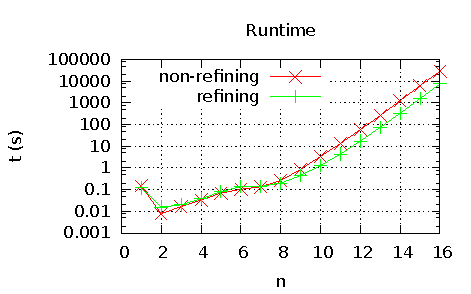
\includegraphics{./graphs/bench_wide_flat_time.pdf}
  \end{minipage}
  \hspace{0.5cm}
  \begin{minipage}[b]{.45\textwidth}
    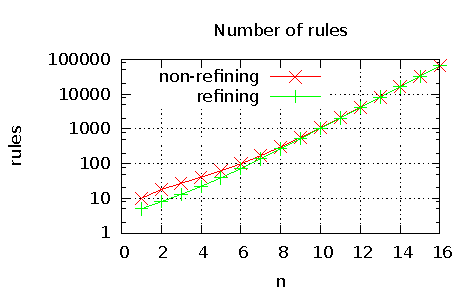
\includegraphics{bench_wide_flat_rules.pdf}
  \end{minipage}
  \caption{Benchmark for mvPDA with high local branching}
  \label{fig:bench-high-local-branching}
\end{figure}

\paragraph{Constant local branching}

For this family, the branching degree from any single state is restricted.
Figure \ref{fig:mvpda-const-local-branching} defines an mvPDA where there
are at most two rules applicable from any state.
The process from $P_0⋅S$ can perform $n$ call transitions, one internal transition
and $n$ return transitions.
These can all be matched by a rule from $Q_0⋅S$, with each $Q_i⋅S$
reachable after $n$ transitions for for $0 ≤ i ≤ n$.
This again leads to an attack rule with a linearly sized right-hand side,
and figure \ref{fig:bench-const-local-branching} confirms the resulting
exponential runtime.

\begin{figure}[H]
  \centering
  \begin{minipage}[b]{.45\textwidth}
    \begin{align*}
      P_i⋅S &\may[c] P_{i + 1}⋅S⋅S && ∀ 0 ≤ i < n \\
      P_n⋅S &\may[i] R_n⋅S \\
      R_{i + 1}⋅S &\may[r] R_i && ∀ 0 ≤ i < n \\
      R_0⋅S &\may[i] P_0⋅S && \text{if }¬ref
    \end{align*}
  \end{minipage}\quad
  \begin{minipage}[b]{.45\textwidth}
    \begin{align*}
      Q_i⋅S &\may[c] Q_i⋅S⋅S && ∀ 0 ≤ i < n \\
      Q_i⋅S &\may[c] Q_{i + 1}⋅S⋅S && ∀ 0 ≤ i < n \\
      Q_i⋅S &\may[i] T_i⋅S && ∀ 0 ≤ i < n \\
      T_i⋅S &\may[r] T_i && ∀ 0 ≤ i < n
    \end{align*}
  \end{minipage}
  \caption{mvPDA with constant local branching}
  \label{fig:mvpda-const-local-branching}
\end{figure}

\begin{figure}[H]
\centering
  \begin{minipage}[b]{.45\textwidth}
    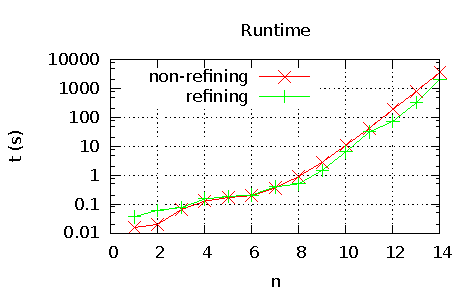
\includegraphics{bench_wide_deep_time.pdf}
  \end{minipage}
  \hspace{0.5cm}
  \begin{minipage}[b]{.45\textwidth}
    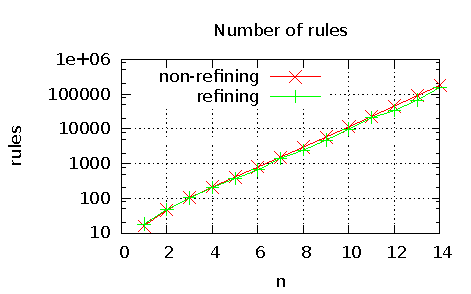
\includegraphics{bench_wide_deep_rules.pdf}
  \end{minipage}
  \caption{Benchmark for mvPDA with constant local branching}
  \label{fig:bench-const-local-branching}
\end{figure}

\paragraph{Constant global branching}

For the next family, the global branching degree is restricted, that
is the maximum width of any attack tree generated.
For that a fixed parameter $k$ is introduced.
Figure \ref{fig:mvpda-const-global-branching} defines
a mvPDA as a variation of the mvPDA from figure \ref{fig:mvpda-const-local-branching},
except here there are only $\mathcal O(k)$ different states reachable from $Q_0⋅S$.

\begin{figure}[H]
  \centering
  \begin{minipage}[b]{.45\textwidth}
    \begin{align*}
      P_i⋅S &\may[c] P_{i + 1}⋅S⋅S && ∀ 0 ≤ i < n \\
      P_n⋅S &\may[i] R_n⋅S \\
      R_{i + 1}⋅S &\may[r] R_i && ∀ 0 ≤ i < n \\
      R_0⋅S &\may[i] P_0⋅S && \text{if }¬ref
    \end{align*}
  \end{minipage}\quad
  \begin{minipage}[b]{.45\textwidth}
    \begin{align*}
      Q_i⋅S &\may[c] Q_i⋅S⋅S && ∀ 0 ≤ i < k \\
      Q_i⋅S &\may[c] Q_{i + 1}⋅S⋅S && ∀ 0 ≤ i < k \\
      Q_i⋅S &\may[i] T_i⋅S && ∀ 0 ≤ i < k \\
      T_i⋅S &\may[r] T_i && ∀ 0 ≤ i < k
    \end{align*}
  \end{minipage}
  \caption{mvPDA with constant global branching}
  \label{fig:mvpda-const-global-branching}
\end{figure}

The results of this benchmark are shown in figure \ref{fig:bench-const-global-branching}
for a number of $k$.
As there were no significant differences between the refining and non-refining
version, only the refining one is shown.
For this family, the runtime is linear with regard to $n$, while
the multiplicative constant is exponential with regard to $k$.

\begin{figure}[H]
\centering
  \begin{minipage}[b]{.45\textwidth}
    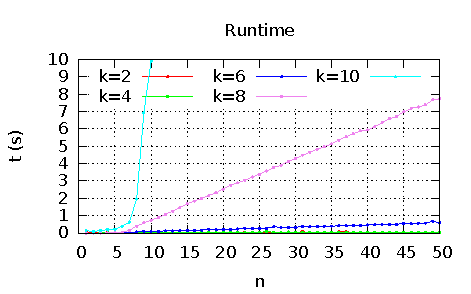
\includegraphics{bench_const_deep_time.pdf}
  \end{minipage}
  \hspace{0.5cm}
  \begin{minipage}[b]{.45\textwidth}
    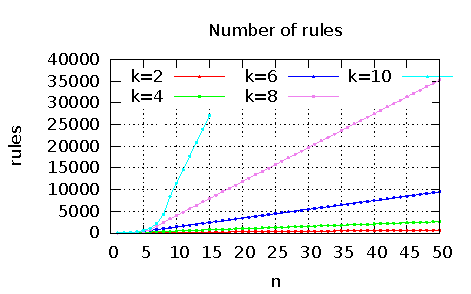
\includegraphics{bench_const_deep_rules.pdf}
  \end{minipage}
  \caption{Benchmark for mvPDA with constant global branching}
  \label{fig:bench-const-global-branching}
\end{figure}

\paragraph{Branching in attacking process}

This family modifies the construction from figure \ref{fig:mvpda-const-global-branching}
and add branching in the attacking process, while keeping branching in the
defending process constant. The resulting construction is shown in figure
\ref{fig:mvpda-attacking-branching}.

\begin{figure}[H]
  \centering
  \begin{minipage}[b]{.45\textwidth}
    \begin{align*}
      P_i⋅S &\may[c] P_i⋅S⋅S && ∀ 0 ≤ i < n \\
      P_i⋅S &\may[c] P_{i + 1}⋅S⋅S && ∀ 0 ≤ i < n \\
      P_n⋅S &\may[i] R_n⋅S \\
      R_{i + 1}⋅S &\may[r] R_i && ∀ 0 ≤ i < n \\
      R_0⋅S &\may[i] P_0⋅S && \text{if }¬ref
    \end{align*}
  \end{minipage}\quad
  \begin{minipage}[b]{.45\textwidth}
    \begin{align*}
      Q_i⋅S &\may[c] Q_i⋅S⋅S && ∀ 0 ≤ i < k \\
      Q_i⋅S &\may[c] Q_{i + 1}⋅S⋅S && ∀ 0 ≤ i < k \\
      Q_i⋅S &\may[i] T_i⋅S && ∀ 0 ≤ i < k \\
      T_i⋅S &\may[r] T_i && ∀ 0 ≤ i < k \\
    \end{align*}
  \end{minipage}
  \caption{mvPDA with branching in attacking process}
  \label{fig:mvpda-attacking-branching}
\end{figure}

The results of this benchmark are shown in figure \ref{fig:bench-attacking-branching}.
Surprisingly, the runtime is polynomial when $k ≤ 3$ and exponential for $k > 3$.
The exponential growth comes from a combination of branching rules from both
sides, leading to attack rules with a right-hand of size in $\mathcal O(nk)$ and runtime
in $2^{\mathcal O(nk)}$.
For $k ≤ 3$, some analysis showed that the combination heuristic could avoid
the exponential growth.

\begin{figure}[H]
\centering
  \begin{minipage}[b]{.45\textwidth}
    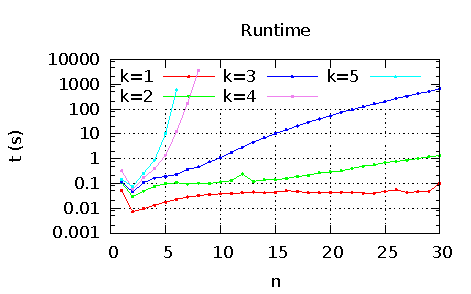
\includegraphics{bench_const_branch_time.pdf}
  \end{minipage}
  \hspace{0.5cm}
  \begin{minipage}[b]{.45\textwidth}
    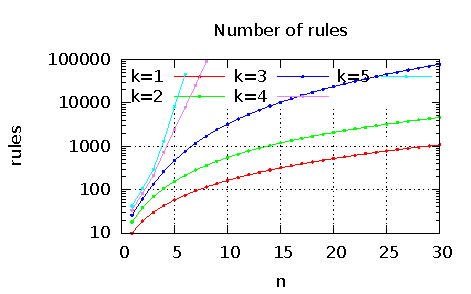
\includegraphics{bench_const_branch_rules.pdf}
  \end{minipage}
  \caption{Benchmark for mvPDA with branching in attacking process}
  \label{fig:bench-attacking-branching}
\end{figure}

\paragraph{Discussion}

The results from the benchmarks show that branching by non-determinism,
either on the attacking and defending side, can lead to exponential runtime
in $2^{\mathcal Ω(n)}$.
This can happen even if the local branching degree is constant.
Branching on both sides even leads to a runtime in $2^{\mathcal Ω(n^2)}$.
If the global branching can be kept constant, however, the runtime is
polynomial.

Further, different orders in which rules are combined can also cause
a change in the runtime. While these are dependent on the input,
there still could be a better heuristic that works better on most inputs.
However, this should be tested on real-world data, of which there is not
much available so far.

